\subsection{Trigger system}

Trigger system in ATLAS is a very essential component, which is responsible for deciding whether to keep a given collision event for later study or not.
In the LHC run-2, higher energy, luminosity and pile-up lead to an large increase of event rate by up to a factor of five comparing to run-1, which causes to a even larger challenge and more strict requirement of trigger system.

The trigger system in run-2 consists of a hardware-based first level trigger (Level-1) and a software-based high level trigger (HLT) \cite{Ruiz-Martinez:2133909}.
As depicted in figure~\ref{fig:trig_syst}, in Level-1, the inputs from coarse granularity calorimeter and muon detector information together with some other subsystems are sent to the Central Trigger Processor to determine Regions-of-Interest (RoIs) in the detector. 
\begin{figure}[!htb]
  \centering
  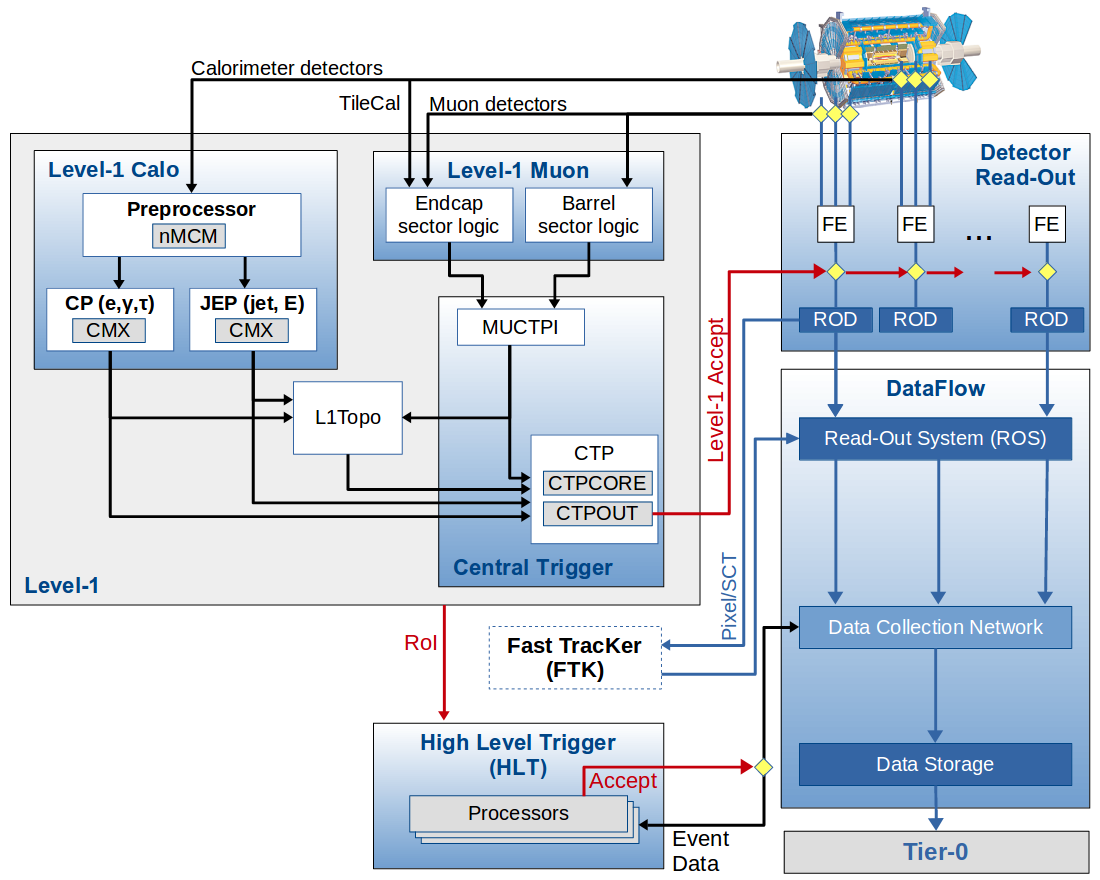
\includegraphics[width=0.9\textwidth]{figures/Detector/tdaq-run2-schematic2017.png}
  \caption{Schematic diagram of the ATLAS trigger and data acquisition system in run-2.}
  \label{fig:trig_syst}
\end{figure}
The event rate can be reduced by Level-1 triggers from 40 MHz to 100 kHz. 
After that, the RoI information from Level-1 is sent to HLT, where more sophisticated selection algorithms are run for regional reconstruction.
The HLT reduces the rate from Level-1 from 100 kHz to about 1 kHz on average.
At the end, the events that accepted by HLT are transferred to local storage at experimental site for offline reconstruction.
Details about Level-1 and HLT trigger systems are described as below:

\textbf{Level-1 trigger}

Substantial upgrades have been delivered in ATLAS Level-1 trigger system for run-2 data taking.
The upgrades took place in both hardware and detector readout, allowing the trigger rate increasing from 70 kHz (in run-1) to 100 kHz (in run-2).
There are two major parts of Level-1 triggers, including Level-1 calorimeter (L1calo) trigger and Level-1 muon (L1mu) trigger.

Level-1 Calorimeter trigger uses the information from the EM and hadronic calorimeters of reduced granularity, to search for photons, electrons, jets and missing transverse energy ($E_{T}^{miss}$).
It can identify an Region-of-Interest (RoI) as a $2 \times 2$ trigger tower cluster in the EM calorimeter as shown in figure~\ref{fig:trig_tower}, 
and $4 \times 4$ or $8 \times 8$ trigger tower for Jet RoIs.
\begin{figure}[!htb]
  \centering
  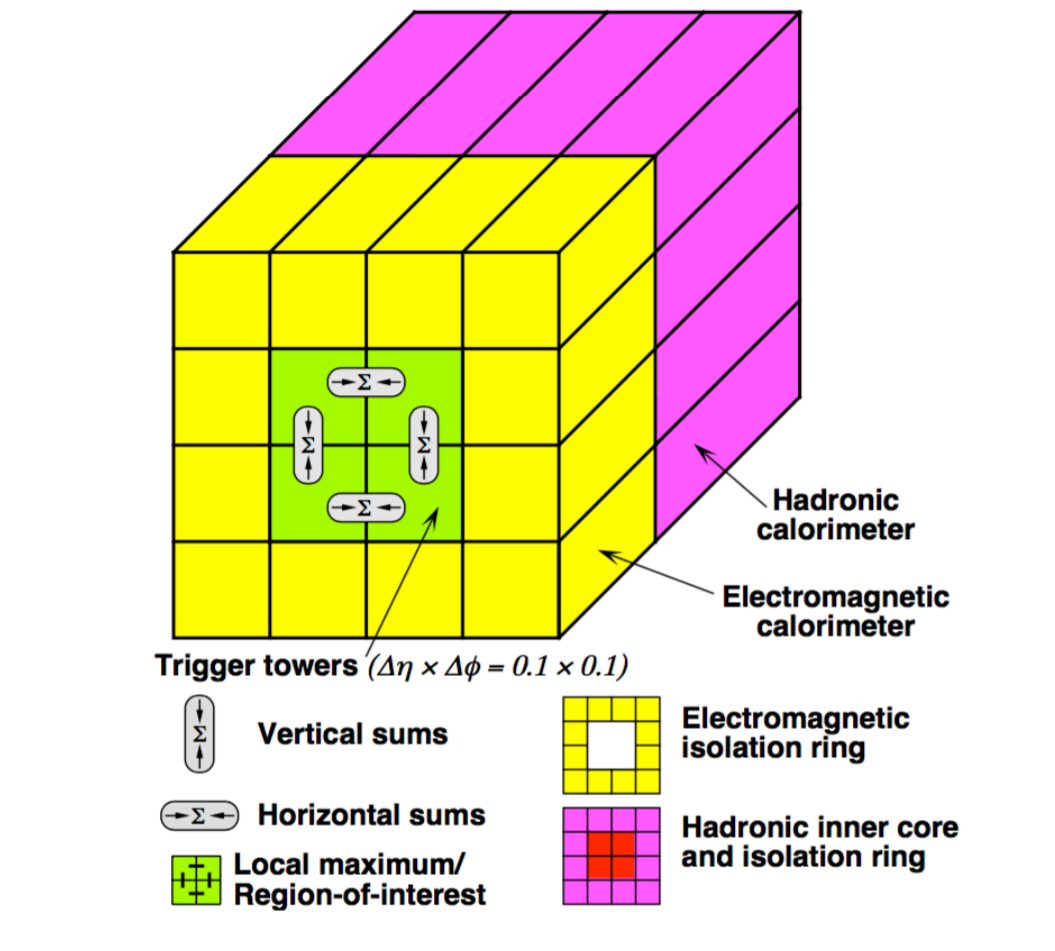
\includegraphics[width=0.6\textwidth]{figures/Detector/trig_tower.png}
  \caption{An examples of L1 calorimeter trigger tower for electron and photon triggers\cite{Pasztor:2063746}.}
  \label{fig:trig_tower}
\end{figure}
One important upgrade was that, the new FPGA-based (field-programmable gate array) Multi-Chip Modules are used to replace the ASICs (application-specific integrated circuits) in the modules used in run-1,
which allows the usage of auto-correlation filters to suppress pile-up.

The Level-1 Muon trigger system includes one barrel section (RPC) and two end-cap section (TGC), which provides fast trigger signals from the muon detectors for the Level-1 trigger decision.
By requiring a coincidence with hits from the innermost muon chambers for muon end-cap trigger, it can reduce the L1$\_$MU15 rate by about 50\% in the region of $1.3 < |\eta| < 1.9$ with only a loss of around 2\% signal efficiency.
In addition, the coverage was extended by around 4\% by installing new chambers in the feet region of the muon detector.

\textbf{High Level Trigger}

In run-1, the Event Filter computer clusters and Level-2 trigger system were separated,
while now in run-2, they have been merged into a single HLT event processing.
The new arrangement helps to reduce the complexity and duplication of algorithm, which leads to a more flexible high level trigger system.
During the long-shutdown between the LHC run-1 and run-2, lots of reoptimizations have been done for trigger reconstruction algorithms as well as the offline analysis selections,
which can improve the efficiency by more than a factor of two in some cases like hadronic tau triggers.
For some triggers, the HLT processing performed within RoIs also allows to aggregate from RoIs to single objects. 
This improvement reduces the CPU processing for events with overlapping RoIs, and the average output rate has been increased from 400 Hz to 1 kHz.

The HLT reconstruction algorithm can be divided into fast and precision online reconstruction steps. 
As illuminated by figure~\ref{fig:trig_alg}, the initial fast reconstruction helps to reduce the event rate, and to seed into precision reconstruction.
Then the final online precision reconstruction is improved and uses offline-like algorithms as much as possible.
In particular, multivariate analysis techniques (based on machine learning) have been introduced online in many aspects.
\begin{figure}[!htb]
  \centering
  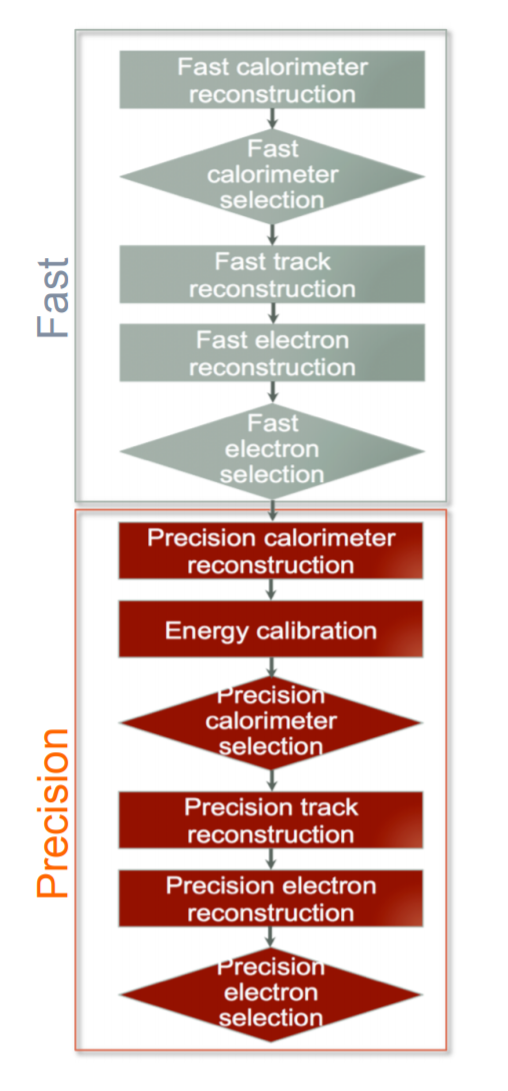
\includegraphics[width=0.5\textwidth]{figures/Detector/trig_alg.png}
  \caption{ The HLT trigger algorithm sequence\cite{Pasztor:2063746}.}
  \label{fig:trig_alg}
\end{figure}
